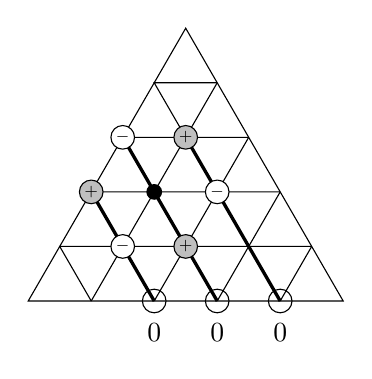
\begin{tikzpicture}[baseline=0cm]
\draw (0,0) -- (4,0) -- (60:4) -- cycle;

\foreach \x in {0.8,1.6,2.4,3.2}
\draw (4,0)++(120:\x) edge (4-\x,0) -- (60:\x) -- (\x,0);

\draw[very thick] (60:2.4) -- +(-60:2.4) ++(0.8,0) -- +(-60:2.4);
\draw[very thick] (60:1.6) -- +(-60:1.6);

\fill (0.8,0) ++(60:1.6) coordinate(v)
	circle[radius=0.1];% ++(0,-0.4)node{$v$};
\foreach \x in {1.6,2.4,3.2}
\draw (\x,0) circle[radius=0.15] ++(0,-0.4)node{$0$};

\foreach \t in {0,120,240}
\draw[fill=white] (v) ++(\t:0.8)node{\tiny$-$} circle[radius=0.15];
\foreach \t in {-60,60,180}
\draw[fill=lightgray] (v) ++(\t:0.8)node{\tiny$+$} circle[radius=0.15];
\end{tikzpicture}